
%%%%%%%%%%%%%%%%%%%%%%% file template.tex %%%%%%%%%%%%%%%%%%%%%%%%%
%
% This is a general template file for the LaTeX package SVJour3
% for Springer journals.          Springer Heidelberg 2010/09/16
%
% Copy it to a new file with a new name and use it as the basis
% for your article. Delete % signs as needed.
%
% This template includes a few options for different layouts and
% content for various journals. Please consult a previous issue of
% your journal as needed.
%
%%%%%%%%%%%%%%%%%%%%%%%%%%%%%%%%%%%%%%%%%%%%%%%%%%%%%%%%%%%%%%%%%%%
%
% First comes an example EPS file -- just ignore it and
% proceed on the \documentclass line
% your LaTeX will extract the file if required
\begin{filecontents*}{example.eps}
%!PS-Adobe-3.0 EPSF-3.0
%%BoundingBox: 19 19 221 221
%%CreationDate: Mon Sep 29 1997
%%Creator: programmed by hand (JK)
%%EndComments
gsave
newpath
  20 20 moveto
  20 220 lineto
  220 220 lineto
  220 20 lineto
closepath
2 setlinewidth
gsave
  .4 setgray fill
grestore
stroke
grestore
\end{filecontents*}
%
\RequirePackage{fix-cm}
%
%\documentclass{svjour3}                     % onecolumn (standard format)
%\documentclass[smallcondensed]{svjour3}     % onecolumn (ditto)
\documentclass[smallextended]{svjour3}       % onecolumn (second format)
%\documentclass[twocolumn]{svjour3}          % twocolumn
%
\smartqed  % flush right qed marks, e.g. at end of proof
%
\usepackage{graphicx}
%
% \usepackage{mathptmx}      % use Times fonts if available on your TeX system
%
% insert here the call for the packages your document requires
%\usepackage{latexsym}
% etc.
%
% please place your own definitions here and don't use \def but
% \newcommand{}{}
%
% Insert the name of "your journal" with
 \journalname{Springers}
%
\begin{document}

\title{Maximum Power Point Tracking in Wind Energy conversion systems using Machine Learning%\thanks{Grants or other notes
%about the article that should go on the front page should be
%placed here. General acknowledgments should be placed at the end of the article.}
}
\titlerunning{MPPT IN WECS using Machine Learning}        % if too long for running head
\author{ Dr. C. Balakrishna Moorthy\and Siddarth Sreeni\and Sahitya Tahiliani }

\institute{Dr. C. Balakrishna Moorthy\at
              Lecturer, BITSPilani, K.K. Birla Goa Campus\\
              Tel.: +832 2580229\\
              Mob.:  +919637356896\\
              \email{cbkmoorthy@gmail.com}  \\
           \and
           Siddarth Sreeni \at
	Student, BITSPilani, K.K.Birla Goa Campus\\
	Mob.: +919400502158\\
             \email{sidda2158@gmail.com}  \\
	\and
	Sahitya Tahiliani \at 
	Student, BITSPilani, K.K.Birla Goa Campus\\
	Mob.: +917038950104\\
	\email{tsahitya105@gmail.com}}

\date{Received: date / Accepted: date}
% The correct dates will be entered by the editor
\maketitle
\begin{abstract}
An efficient and feasible algorithm to extract the maximum power point in Wind Energy Conversion Systems has been done by implementing Machine Learning (ML) into Perturb and Observe(P\&O) algorithm. In this paper, the advantages of using ML have been explained and verified. The proposed model consists of a charger controller circuit and a self excited DC generator. This model uses instantaneous measurement of wind speeds, humidity, temperature, pressure and generator speed and estimates a Maximum Power Point (MPP). From this estimated power point, the controller follows quick perturbation to calculate the accurate MPP and is corrected and is used as training data for further predictions in the next iterations. The controller learns from this training set and estimates the MPP closer to the Maximum Achievable Power Point and is again corrected and recorded.With the progress in time, the estimation of the maximum power point becomes accurate and decreases the time in further perturbation required for correction. This algorithm thus adapts to the versatile environment conditions. The simulation results of the proposed method has been described in this paper.

\keywords{Wind Energy Conversion Systems \and Wind Power Generation \and Power generation control \and Maximum Power Point Tracking \and Perturb and Observe \and Hill climb Search \and Machine Learning \and Artificial Intelligence}

\end{abstract}

\section{Introduction}
\label{intro}
Wind Energy Conversion Systems (WECS) are of major importance in recent days\cite{RefJ1}. Majority of the energy requirements in today’s world are met with fossil fuels which are costly, non-renewable and pollute the environment. Hence, there is a need to change to green energy resources. A lot of research is carried out in this area to find alternative energy resources that are renewable and can be easily harnessed. Existing such resources are solar and wind energy. Wind energy is a good alternative to become environmental friendly and ecologically aware. Almost all regions of our country gets enough wind to produce massive amount of wind energy[2] and the need to optimise that process poses as a question.
Hence, an effective mechanism is required to efficiently harness maximum wind energy power. Since wind speed is continuously changing, it is difficult to extract a continuous and maximum power. Hence, there is a need for WECS to be carried out efficiently. Thus, an efficient and cost-effective system which is able to transfer the maximum power is required. Any WECS essentially consists of a Wind Turbine, Charger Controllers and an Inter-Connection apparatus to supply the generated power from the wind to the transformers for further distribution. During windy periods, the wind cuts the blades of the turbine fan and causes the blades to rotate which in turn generates a torque supply to the generator. The generators uses variable loads to efficiently use the supply and maximize the power output. Wind energy power output can be analyzed based on the P-V curve .A graph of the Power Vs Voltage characteristics under a constant wind speed is shown in Figure.1.
\begin{center}
\begin{figure}
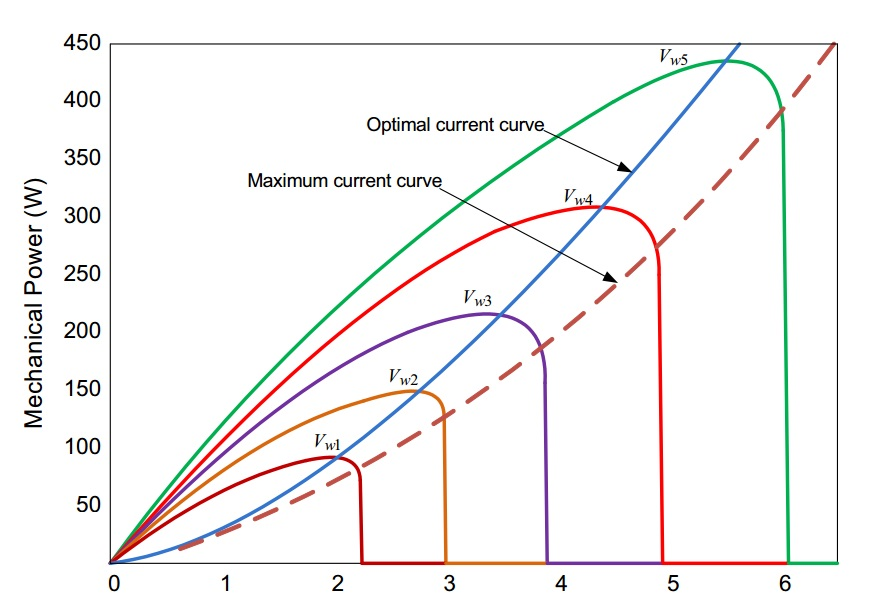
\includegraphics[width=10cm,height=20cm,keepaspectratio]{1.png}
\caption{The Power Vs Current under constant wind speed.[1]}
\label{Fig:1}    
\end{figure}

\end{center}
A load impedance is required for the generator to change the values of voltage and thus track the maximum power at each wind speed. But, since the graph plotted keeps shifting from its original position as the wind speed is changing continuously, this fluctuates the peak point of power. Therefore, the load impedance needs to be changed again in order to get the maximum power characteristic values for voltage and thus current again. The process is known as Maximum Power Point Tracking (MPPT).
MPPT is carried out by designing efficient charger controllers to extract maximum power from the WECS. The charger controller is coded with an algorithm to fluctuate and control the load impedances given to the generator thereby controlling the power output. Various methods like Perturb and Observe (P and O)[2] , method of Incremental Conductance[3], method of Fractional Voltage[4], Neural Network[5] and fuzzy logic control [6] , etc. are being used to mechanize charger controllers and generate suitable power outputs. All these methods have been compared on the basis of their complexity, efficiency, performance, etc. and have been plotted in Table.1.


\begin{center}
\begin{table}[hbtp]
% table caption is above the table

\label{Table:1}       % Give a unique label
% For LaTeX tables use
\caption{Comparison of MPPT techniques on different parameters.[5]}



\begin{tabular}{lllll}
\hline\noalign{\smallskip}

Technique & Convergence Speed & Complexity &Tuning & Parameters  \\
\noalign{\smallskip}\hline\noalign{\smallskip}
Peturb and Observe & Varies & Low &  No & Voltage \\
Incremental Conductance  &  Varies & Medium & No & Voltage,Current \\
Fractional Voltage & Medium & Low & Yes & Voltage \\
Fractional Current & Medium & Medium & Yes & Current \\
Fuzzy Logic Control & Fast & High & Yes & Varies \\
Neural Network & Fast & High & Yes & Varies \\
\noalign{\smallskip}\hline

\end{tabular}
\end{table}
\end{center}
In this article, an alternative approach to the existing methods has been suggested overcoming a lot of limitations in terms of efficiency and performance. A separately excited DC generator Fig.2. has been used for simulation.
\begin{center}
\begin{figure}
 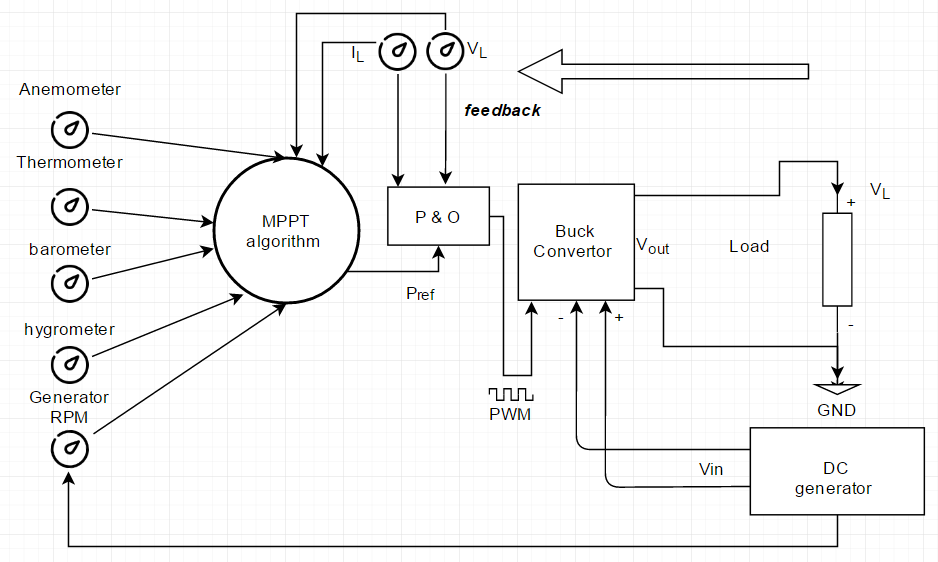
\includegraphics[width=10cm,height=20cm,keepaspectratio]{2.png}
\caption{Load tests on a Separately excited DC generator. [7]}
\label{Fig:2}    
\end{figure}
\end{center}
\section{System Model}
\label{sec:1}
Figure 3. describes the working of the  proposed wind energy conversion system.The system consists of a wind turbine coupled with a separately excited  DC generator.The buck converter is coupled with the DC generator and acts as a DC to DC converter that controls the ratio of input and output voltage by a PWM (Pulse Width Modulation) signal from the MPPT charger controller.
\begin{center}
\begin{figure}
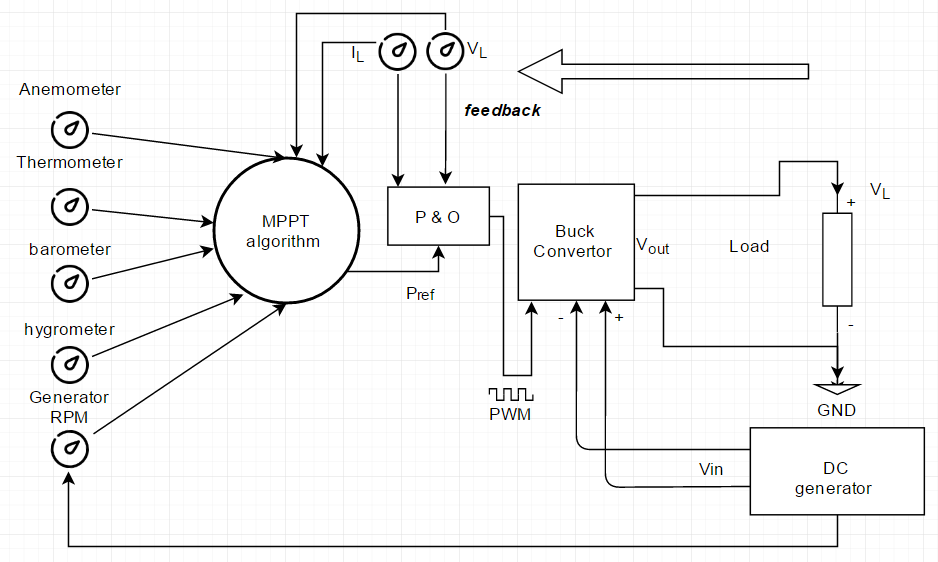
\includegraphics[width=10cm,height=20cm,keepaspectratio]{3.png}
\caption{The configuration of wind energy conversion system}
\label{Fig:3}    
\end{figure}
\end{center}
\subsection{Separately excited DC generator Model:}
The wind energy conversion systems convert the kinetic energy of the wind into electrical energy.The mechanical power $P_m$ fed to the wind turbine is described as kinetic energy(KE) of the wind turbine rotor blade per unit time[8]:


\begin{equation}
P_m =\frac{KE}{t} = \frac{1}{2} \rho  Av^3
\end{equation}

where ,
$\rho$ is the air density
$A$ is the area swept by the rotor blade 
$v$ is the wind velocity (m/s)
This is ideal power fed to the wind turbine.But there is a theoretical limit to which this power can be utilised in practice.This limit is governed by Betz’s law[9],which talks about the maximum power that can be extracted from the wind, independent of the design of a wind turbine in open flow.According to Betz's law, no wind turbine can capture more than 59.3\% of the kinetic energy in wind.
The power generated by the wind turbine depends on the efficiency factor, also known as coefficient of  performance Cp($\lambda $,$\beta$) of the wind turbine which depends on  tip speed ratio ($lambda$) and pitch angle ($\beta$).
The tip speed ratio is the ratio of  the turbine speed to the wind speed and is given by[10]:

\begin{equation}
\lambda=\omega \frac{R}{V}
\end{equation}

where, $\omega$ is the angular speed of the turbine and R is the radius of the turbine.Hence,the actual power generated by the wind turbine is:

\begin{equation}
P=C_p(\lambda,\beta)P_m = \frac{1}{2}C_p(\lambda,\beta) \rho  Av^3
\end{equation}
The coefficient of  performance has a theoretical value of 0.593 (Betz’s Law)[9].The turbine’s coefficient of performance is a nonlinear function and is expressed by[11]: 

\begin{equation}
C_p(\lambda,\beta) = 0.5 ( 116 \frac{1}{\lambda_i} - 0.4 \beta - 5) e^\frac{-21}{\lambda_i}
\end{equation}
Where,
\begin{equation}
\frac{1}{\lambda_i} = \frac {1}{\lambda + 0.08 \beta} - \frac{0.035}{1+\beta^3}
\end{equation}

The characteristic curve for coefficient of  performance Cp($\lambda$,$\beta$) vs tip speed ratio($\lambda$) for various values of the pitch angle ($\beta$) is shown below in Fig 4:

\begin{center}
\begin{figure}
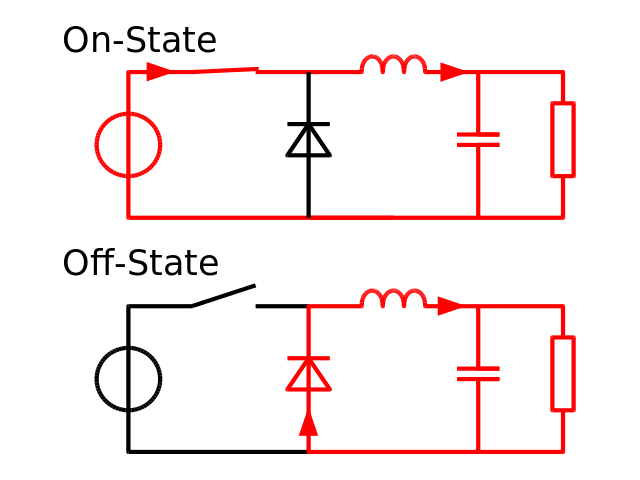
\includegraphics[width=10cm,height=20cm,keepaspectratio]{4.png}
\caption{$C_p(\lambda,\beta)$ vs $\lambda$ characteristic curve for different $\beta$. [12]}
\label{Fig:4}    
\end{figure}
\end{center}

\subsection{Buck Convertors}
Buck Converters[13] are used for stepping down DC voltage,by stepping down voltage from the input supply to the output y work on thesupply(generator load).The principle of  SMPS(switched mode power supply),essentially containing components like diode,transistor and capacitor/inductor(energy storing elements).Buck Converters are highly efficient (upto 90\%),making them useful for a lot of computational operations as well.The principle of  a buck converter is basically control of  the inductor current by the means of  switches(usually a transistor/diode) thereby stepping down the supply voltage.A basic circuit diagram of  buck converter is shown in Fig.5.
\begin{center}
\begin{figure}
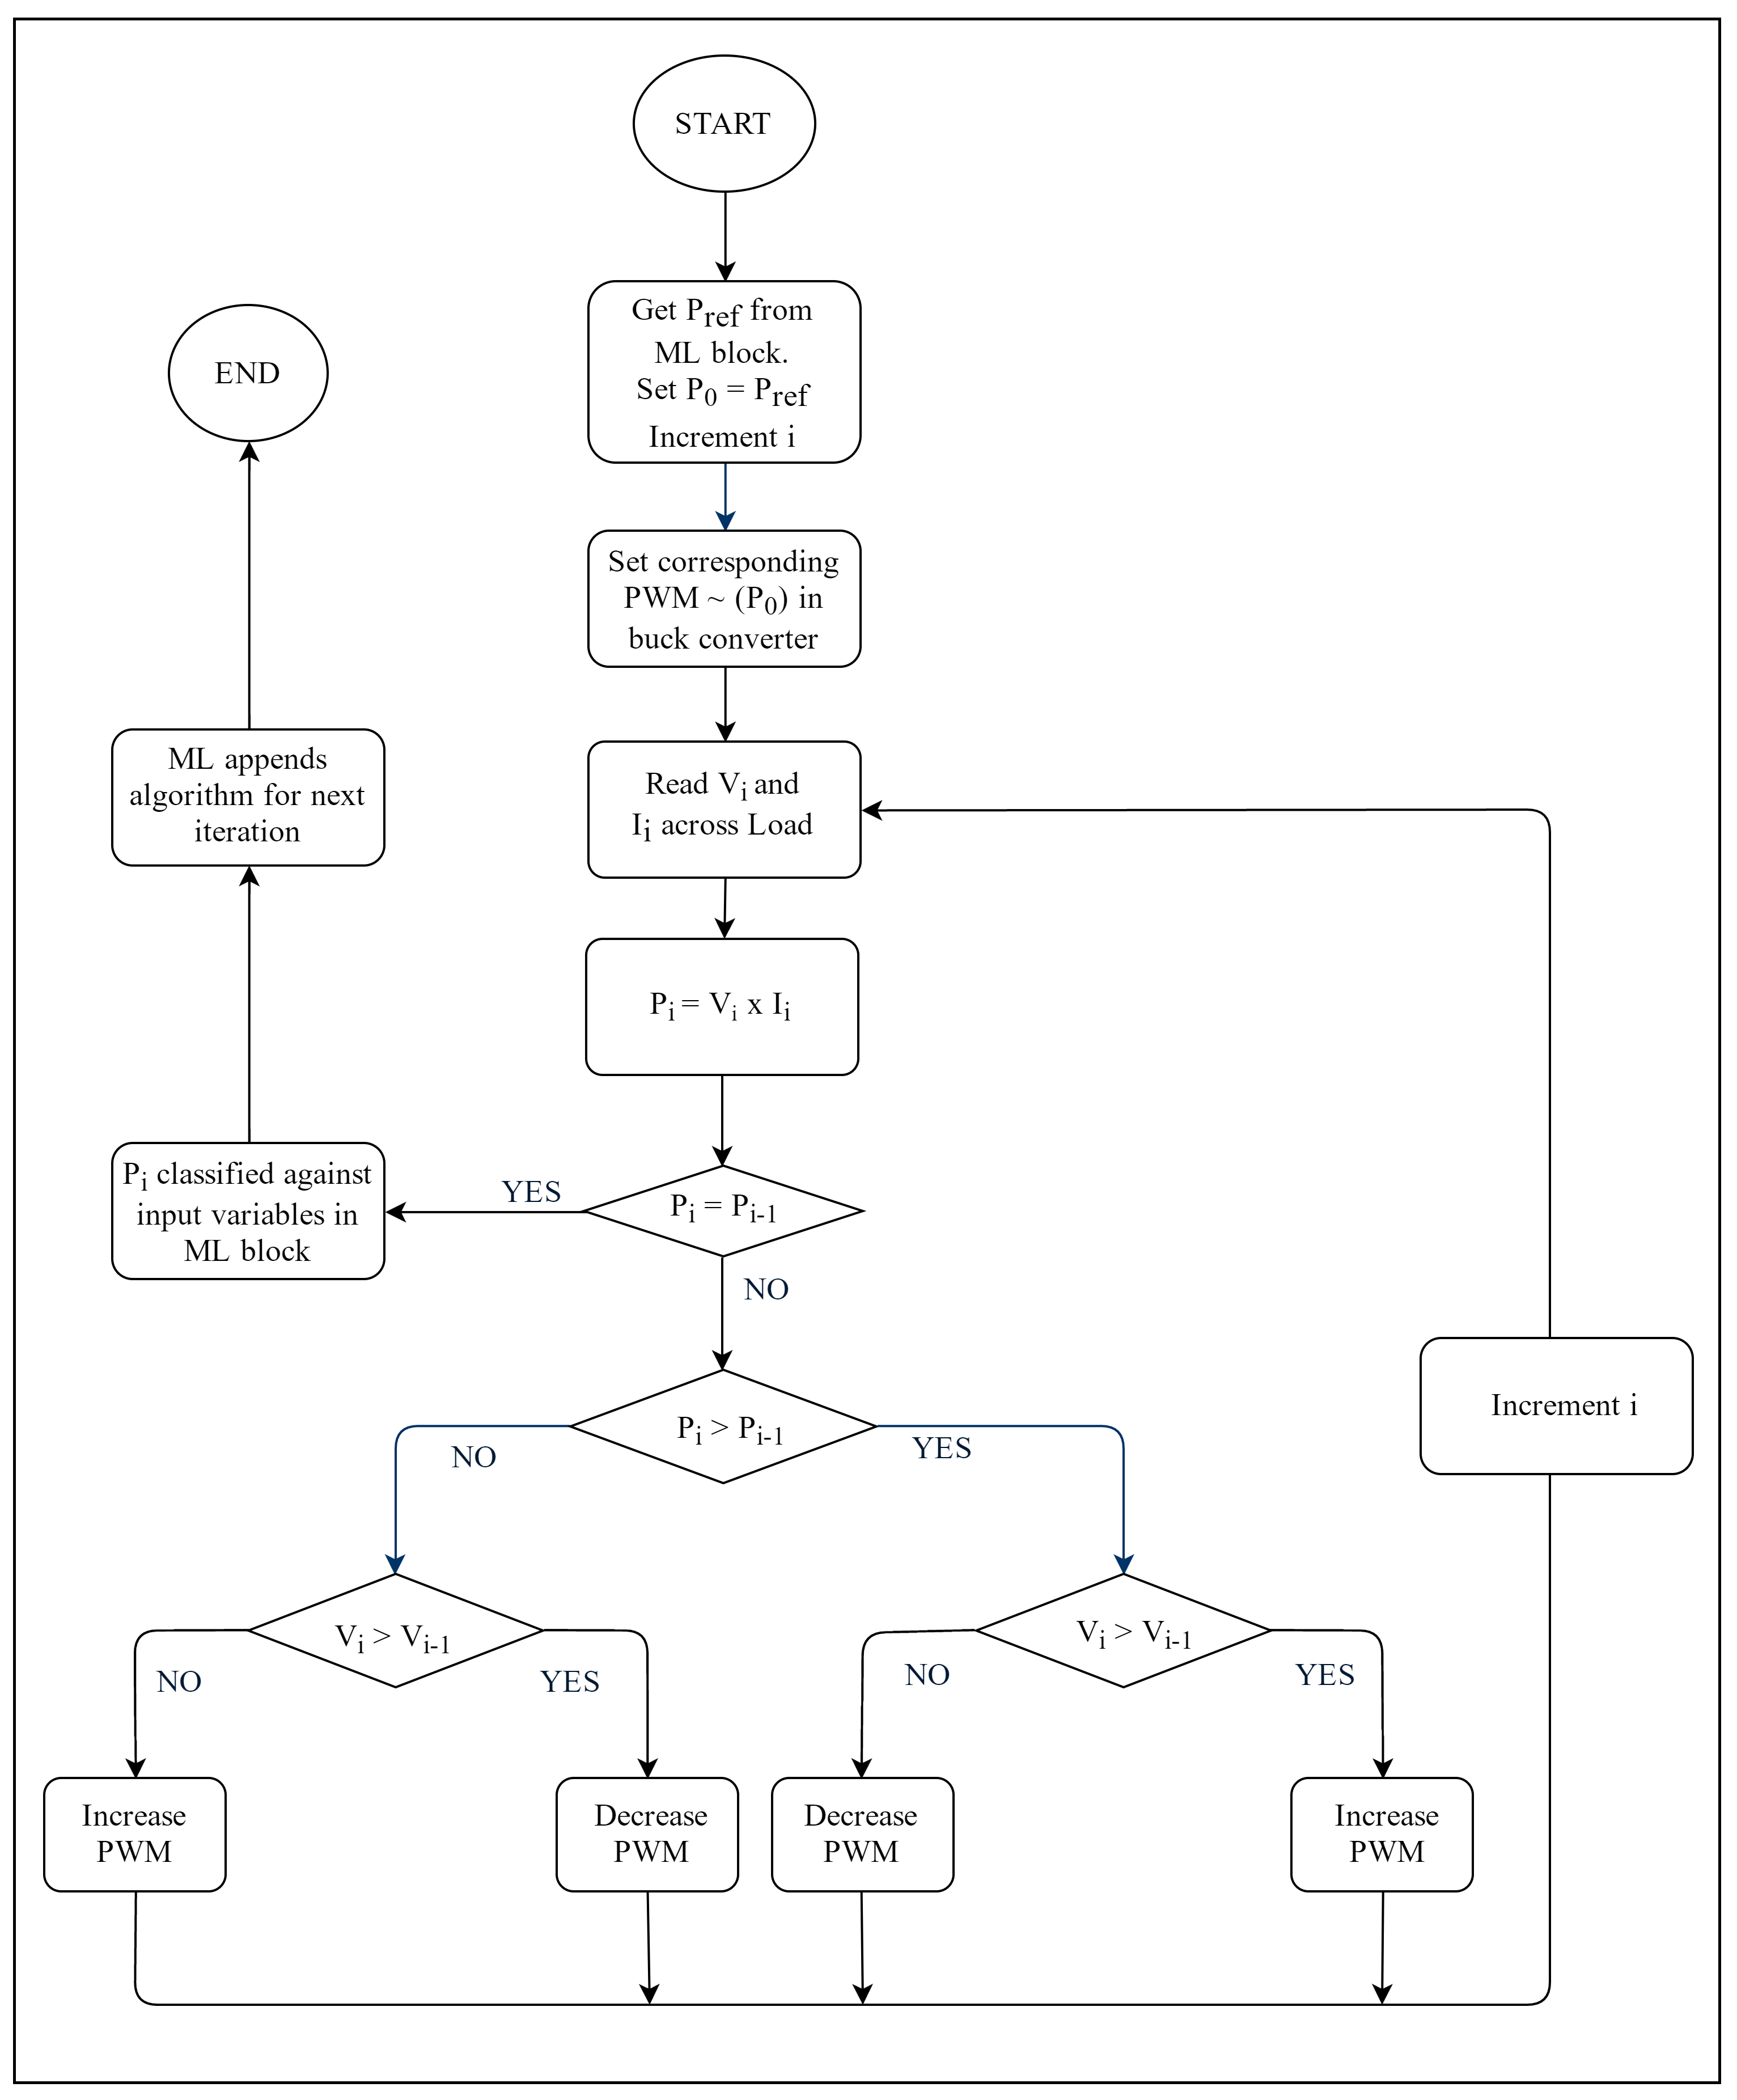
\includegraphics[width=10cm,height=20cm,keepaspectratio]{5.png}
\caption{ A circuit showing modelling of buck converters[13]}
\label{Fig:5}    
\end{figure}
\end{center}
\subsection{Peturb and Observe}
Perturb and Observe (P\&O) also known as the hill climbing method(HCS) is the most simplistic and efficient method for maximum power point tracking in wind-energy conversion systems [14],[15] .In this method,the controller adjusts the output voltage of the separately excited DC generator by varying the duty cycle of the buck converter, and measures the rise and fall in power continuously.If there is an increment in the power on increasing the duty cycle,then the duty cycle is increased further in the same direction.If there is a decrement in power,then the direction of duty cycle is reversed and the process is repeated in the opposite direction until there is no further rise in power. Hence,the characteristic parameters of this point being the maximum power point are recorded and the optimum power is generated using them.This is call the Perturb and observe methodology and is one of the most frequent and commonly used methods in the industry due to its ease of implementation.A flow chart depicting the change in duty cycles as per the power requirements has been shown in the Fig.6.

\begin{center}
\begin{figure}
\includegraphics[width=10cm,height=20cm,keepaspectratio]{6.png}
\caption{Flowchart depicting P\&O algorithm}
\label{Fig.6}    
\end{figure}
\end{center}

\subsection{MPPT Algorithm}
The proposed method is a modified approach to Perturb and Observe or Hill climb Search algorithm. The process of Machine Learning is similar to data mining, however the obtained results and conclusions from the older data are used to estimate results for the new data. This so called supervised learning technique is being used in this paper. The Machine learning algorithm  used in the system estimates a power point close to the actual MPP using a regression model based on earlier values and inputs. It is a causal system. The current wind-speed, temperature, pressure and humidity are taken to estimate the maximum power point. This model generates an algorithm and recognizes patterns in the formation of the MPP(s). As time progresses by, the feedback updates the estimation algorithm. The system recognizes more patterns and thus improves the regression model. A graph between actual MPP and predicted MPP has been plotted in Fig 7.

This model uses a combination of a linear regression algebra to detect patterns and a feedback mechanism based on $V_L$ and $I_L$ obtained from the previous MPP(s) to supervise the next estimation.


\begin{equation}
\phi =F_t( \phi_0 .... \phi_{t-1}) 
\end{equation}

where,$\phi(t)$ is the MPP at time $t$  and $F_t$ is the estimation function at time $t$.  The obtained result is  passed on to the next block as $V_{ref}$ and from here the algorithm follows normal hill climb search to obtain the MPP Ptusing a synchronous Buck DC- DC convertor.  The Machine learning block ( MPPT Algorithm) given in the Fig 3. uses  instantaneous measurements from Anemometers, Hygrometers, Barometers,Thermometers, and the generator RPM to decide on the estimation. 

A linear regression model is generalized by the following formula. The prediction of $Y$ is computed by[16],


\begin{equation}
Y^1= b_0 + b_1 X_{1i} + ... + b_k X_{ki}
\end{equation}

The $b$ values are called regression weights and are computed in a way that minimizes the sum of squared deviations (Eq.8), here, there are $k$ predictor variables.


\begin{equation}
\sum_{i= 1 }^{N} (Y_i - Y^1_i)^2
\end{equation}

\begin{center}
\begin{figure}
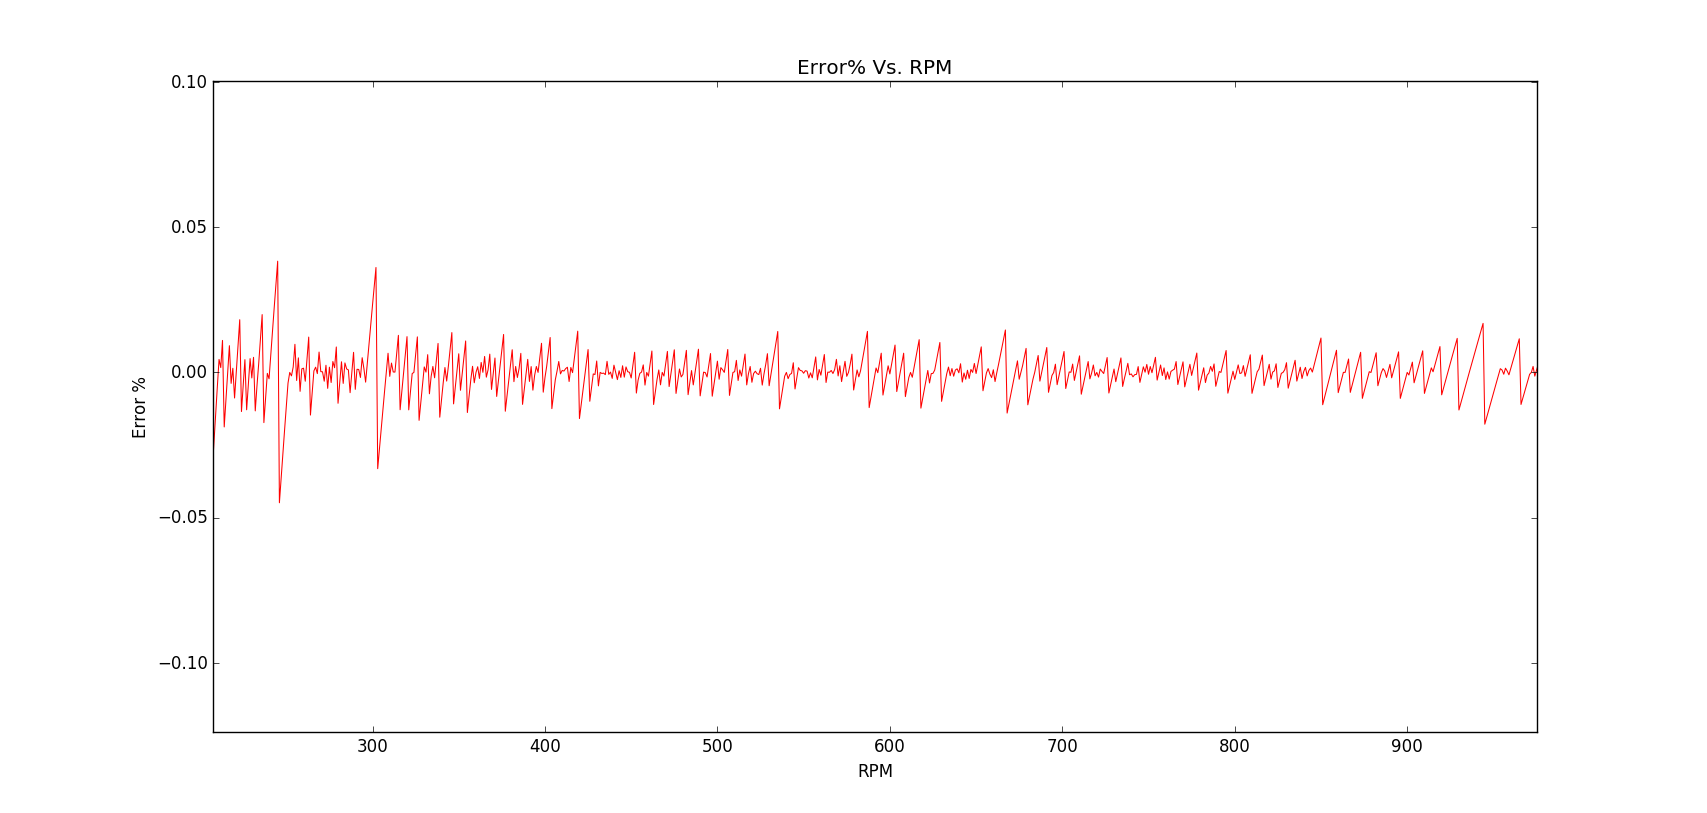
\includegraphics[width=10cm,height=20cm,keepaspectratio]{7.png}
\caption{Power Estimated $\phi_t$ (blue) and available $P_t$(red)}
\label{Fig:7}    
\end{figure}
\end{center}

The prediction of function $F_t$  to the actual MPP $\phi_t$ is much more accurate to$ F_{t-1}$. Which is why, there is an understanding of learning and intelligence. 

\begin{center}
\begin{figure}
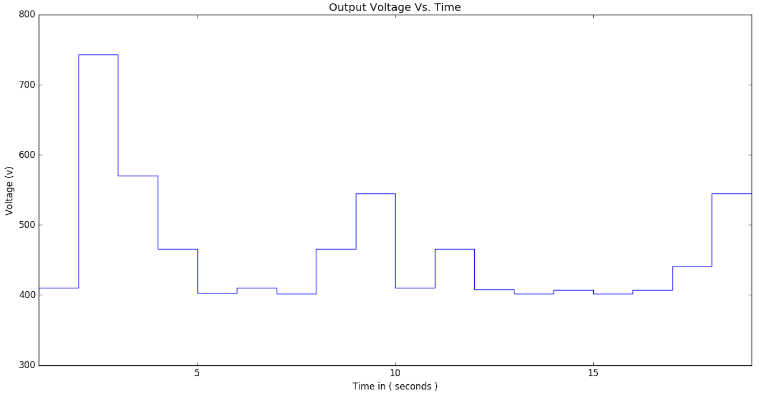
\includegraphics[width=10cm,height=20cm,keepaspectratio]{8.png}
\caption{ Percentage Error for different rpm of the generator at time t=1000}
\label{Fig:8}    
\end{figure}
\end{center}

The Figures 9-10 shows the dynamic responses of the PV system driven by the MPPT algorithm in terms of generated output voltage and current.When $t$ is sufficient enough, the percentage difference $\Delta$  between actual MPP $P_t$ and $\phi_t$  will become lesser as time progresses. This has been verified and under simulation, the predicted errors were less. In this domain, Machine learning overcomes over fitting that usually occurs in other AI algorithms such as Artificial Neural Networks (ANN) and logical control systems. As a validation dataset (P\&O) is fed back after each iteration into the training data, this limits the errors from increasing.

\begin{equation}
\Delta  = 100 ( \frac{P_t - \phi_t}{\phi_t})\%
\end{equation}

\begin{center}
\begin{figure}
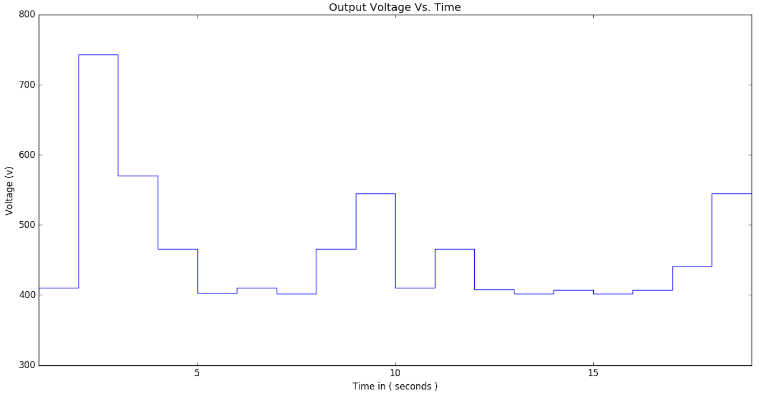
\includegraphics[width=10cm,height=20cm,keepaspectratio]{9.png}
\caption {Output Voltage based MPPT control}
\label{Fig:9}    
\end{figure}
\end{center}

\begin{center}
\begin{figure}
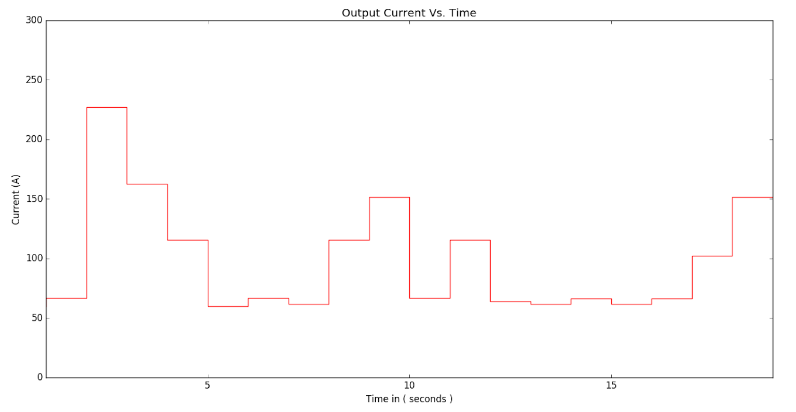
\includegraphics[width=10cm,height=20cm,keepaspectratio]{10.png}
\caption {Output Current based MPPT control}
\label{Fig:10}    
\end{figure}
\end{center}

Finally, the performance of the modified MPPT control using Machine Learning technique can be detected according to the efficiency,

\begin{equation}
\eta_t  = (100 - \Delta_{max}^t)\%
\end{equation}

As $\eta$ depends on time, the efficiency increases and reach a value close to 100\% with time. From Fig 6. , The overall tracking efficiency of the proposed MPPT system at t=1000s is greater than 99.48\% for any climatic conditions, hence the effectiveness of the proposed MPPT control method is highly ensured as required.

\section{Conclusion and Perspective:}
In this paper, an intelligent method to track the maximum power point under rapid changes of weather conditions has been developed and tested. A Python based simulation of a wind turbine energy conversion system with a dc load stage has been carried out to validate the proposed MPPT method. The results showed  that the proposed MPPT method tracked the MPP with negligible oscillations. Observations show that the performance and accuracy of the proposed method is not influenced by the load variations at all. A slight variation is observed when unexpected wind speeds occur, but after a very small amount of time the system moves smoothly to the MPP and is recorded. The main advantages of the developed MPPT control method are fast convergence to the MPP, high efficiency, robustness and its possibility to implement easily. The system is a modified algorithm of P\&O and can be added as an extra block to the existing P\&O equipments indicating its ease of setting up. Further work is being conducted on the overall system design and experimental implementation.


\begin{thebibliography}{}
\bibitem{RefJ0}

M. G. Villalva, J. R. Gazoli, and E. R. Filho, “Comprehensive Approach to Modeling and Simulation of Photovoltaic Arrays,” IEEE Trans. Power Electron., vol. 24, no. 5, pp. 1198–1208, 2009.
\bibitem{RefJ1}
M. A. Elgendy, B. Zahawi, and D. J. Atkinson, “Evaluation of perturb and observe MPPT algorithm implementation techniques,” in 6th IET International Conference on Power Electronics, Machines and Drives (PEMD 2012), 2012.
\bibitem{RefJ2}
T. Boutabba, S. Drid, L. Chrifi-Alaoui, M. Ouriagli, and M. E. H. Benbouzid, “dSPACE real-time implementation of maximum power point tracking based on ripple correlation control (RCC) structure for photovoltaic system,” in 2016 5th International Conference on Systems and Control (ICSC), 2016.
\bibitem{RefJ3}
S. M. Ferdous, M. A. Mohammad, N. Farhan, A. M. Saleque, and M. A.Z.M.Shahriar, “Design and simulation of an open voltage algorithm based maximum power point tracker for battery charging PV system,” in 2012 7th International Conference on Electrical and Computer Engineering, 2012.
\bibitem{RefJ4}
T. Esram, E. Trishan, and P. L. Chapman, “Comparison of Photovoltaic Array Maximum Power Point Tracking Techniques,” IEEE Trans. Energy Convers., vol. 22, no. 2, pp. 439–449, 2007.
\bibitem{RefJ5}
I. H. Altas, Fuzzy Logic Control in Energy Systems with MATLAB. 2017.
\bibitem{RefJ6}
D. P. Kothari, Electric Machines (Sigma). Tata McGraw-Hill Education, 2006.
\bibitem{RefJ7}
A. Soetedjo, S. Aryuanto, L. Abraham, and W. P. Mulayanto, “Modeling of wind energy system with MPPT control,” in Proceedings of the 2011 International Conference on Electrical Engineering and Informatics, 2011.
\bibitem{RefJ8}
A. Betz, Introduction to the Theory of Flow Machines. Elsevier, 2014.
\bibitem{RefJ9}
H. Yokoyama, Y. Hiroyuki, T. Fujio, and N. Shoji, “Tip speed ratio control of wind turbine generating system connected in series,” in 2011 International Conference on Electrical Machines and Systems, 2011.
\bibitem{RefJ10}
M. Azzouz, A. Maher, E. Abdel-Latif, and E. Hasan, “Adaptive critic design-based regulation of the DC-bus voltage in wind energy conversion systems,” in 49th IEEE Conference on Decision and Control (CDC), 2010.
\bibitem{RefJ11}
C. Viveiros, R. Melício, J. M. Igreja, and V. M. F. Mendes, “Supervisory control of a variable speed wind turbine with doubly fed induction generator,” Energy Reports, vol. 1, pp. 89–95, 2015.
\bibitem{RefJ12}
M. Brown and B. Marty, “Switching Power Supply Topologies,” in Practical Switching Power Supply Design, 1990, pp. 17–42.
\bibitem{RefJ13}
E. Koutroulis and K. Kalaitzakis, “Design of a maximum power tracking system for wind-energy-conversion applications,” IEEE Trans. Ind. Electron., vol. 53, no. 2, pp. 486–494, 2006.
\bibitem{RefJ14}
H. Gitano, G. Horizon, T. Soib, and K. Mohammad, “Design and Testing of a Low Cost Peak-Power Tracking Controller for a Fixed Blade 1.2 kVA Wind Turbine,” in 2007 Compatibility in Power Electronics, 2007.
\bibitem{RefJ15}
T. Hill, P. Lewicki, and P. Lewicki, Statistics: Methods and Applications : a Comprehensive Reference for Science, Industry, and Data Mining. StatSoft, Inc., 2006.





% etc
\end{thebibliography}

\end{document}
% end of file template.tex

